% ==============================================================================
% DOCUMENTO PRINCIPAL - LATEX
% Proyecto: SIGC-CUSCO | Proceso de Desarrollo e Incremento 1
% Asignatura: Ingeniería de Software I - UNSAAC
% ==============================================================================

\documentclass[12pt,a4paper]{article}

% ==============================================================================
% CONFIGURACIÓN DE PAQUETES - LATEX
% SIGC-CUSCO | Informe de Proceso e Incrementos de Desarrollo
% ==============================================================================

\usepackage[utf8]{inputenc}
\usepackage[T1]{fontenc}
\usepackage[spanish, es-tabla, es-nodecimaldot]{babel}
\spanishdeactivate{"}
\usepackage{csquotes}

\usepackage[margin=2.54cm, headheight=18pt]{geometry}

\usepackage{mathptmx}
\usepackage{amssymb}
\usepackage{setspace}
\onehalfspacing

\usepackage{graphicx}
\graphicspath{{./}{imagenes/}{./imagenes/}}
\usepackage{float}
\usepackage{booktabs}
\usepackage{tabularx}
\usepackage{array}
\usepackage{caption}

\usepackage[table]{xcolor}
\definecolor{colorRojoAlerta}{RGB}{180, 0, 0}
\definecolor{fondoRojoAlerta}{RGB}{255, 243, 243}

\usepackage{enumitem}

\usepackage{fancyhdr}
\pagestyle{fancy}
\fancyhf{}
\fancyhead[L]{\small\itshape UNSAAC -- Ingeniería de Software I}
\fancyhead[R]{\small\itshape SIGC-CUSCO -- Informe de Desarrollo}
\fancyfoot[C]{\thepage}
\renewcommand{\headrulewidth}{0.4pt}
\renewcommand{\footrulewidth}{0pt}

\usepackage{xurl}
\usepackage{hyperref}
\usepackage[spanish]{cleveref}
\hypersetup{
    colorlinks=true,
    breaklinks=true,
    linkcolor=blue!75!black,
    urlcolor=blue!75!black,
    pdftitle={Informe de Desarrollo - SIGC-CUSCO},
    pdfauthor={Choquenaira, Yaranga, Ccama}
}

\usepackage{microtype}
\emergencystretch=2.5em

\setlength{\parindent}{0.6cm}
\setlength{\parskip}{0.18em}

\newcolumntype{Y}{>{\raggedright\arraybackslash}X}
\newcolumntype{P}[1]{>{\raggedright\arraybackslash}p{#1}}

% Entorno estructurado para evidencias pendientes en rojo
\newenvironment{cajaevidencia}[1]{%
    \par\vspace{0.3cm}
    \noindent\begingroup\color{colorRojoAlerta}%
    \rule{\linewidth}{1pt}\par\vspace{0.15cm}%
    \noindent\textbf{[EVIDENCIA PENDIENTE: #1]}\par\vspace{0.15cm}%
}{%
    \par\vspace{0.15cm}\noindent\rule{\linewidth}{1pt}%
    \endgroup\par\vspace{0.3cm}%
}


\begin{document}
\hypersetup{pageanchor=false}

% 1. Portada Oficial UNSAAC
\begin{titlepage}
    \centering
    \vspace*{0.2cm}
    
    {\fontsize{13}{16}\selectfont \textbf{UNIVERSIDAD NACIONAL DE SAN ANTONIO ABAD DEL CUSCO}}\\[0.25cm]
    {\fontsize{11}{14}\selectfont \textbf{FACULTAD DE INGENIERÍA ELÉCTRICA, ELECTRÓNICA, INFORMÁTICA Y MECÁNICA}}\\[0.25cm]
    {\fontsize{11}{14}\selectfont \textbf{ESCUELA PROFESIONAL DE INGENIERÍA INFORMÁTICA Y DE SISTEMAS}}\\[0.4cm]
    
    
\includegraphics[width=3.4cm]{escudo.png}\\[0.4cm]
    
    {\fontsize{13}{16}\selectfont \textbf{INFORME DE INGENIERÍA DE SOFTWARE}}\\[0.15cm]
    {\fontsize{12}{15}\selectfont \textbf{PROCESO DE DESARROLLO Y PRIMER INCREMENTO}}\\[0.25cm]
    \rule{\textwidth}{1.2pt}\\[0.2cm]
    {\fontsize{13}{16.5}\selectfont \textbf{``SISTEMA INTEGRAL DE GESTIÓN DE CAPACITACIONES (SIGC-CUSCO)''}}\\[0.15cm]
    \rule{\textwidth}{1.2pt}\\[0.5cm]
    
    \begin{minipage}{0.92\textwidth}
        \setstretch{1.2}
        \textbf{Asignatura:} Ingeniería de Software I\\[0.2cm]
        \textbf{Docente de Teoría:} Prof. Jisbaj Gamarra Salas\\[0.2cm]
        \textbf{Docente de Prácticas:} Ing. Lisha Sabah Diaz Caceres\\[0.2cm]
        \textbf{Integrantes:}\\[0.15cm]
        \hspace*{0.4cm}\textbullet\quad Choquenaira Quispe, Noe Franklin \hfill 133962\\[0.12cm]
        \hspace*{0.4cm}\textbullet\quad Yaranga Achahui, Aldo \hfill 103179\\[0.12cm]
        \hspace*{0.4cm}\textbullet\quad Ccama Enriquez, Carolay \hfill 210921
    \end{minipage}\\[0.7cm]
    
    \vfill
    {\textbf{Cusco -- Perú}}\\[0.1cm]
    {\textbf{2026}}
\end{titlepage}


% 2. Tabla de Contenidos
\newpage
\hypersetup{pageanchor=true}
\pagenumbering{roman}
{
    \hypersetup{linkcolor=black}
    \begin{spacing}{0.95}
    \tableofcontents
    \end{spacing}
}
\newpage
\pagenumbering{arabic}

% 1. Datos generales del proyecto
\section{Datos generales del proyecto}

El proyecto \textbf{Sistema Integral de Gestión de Capacitaciones (SIGC-CUSCO)} es una plataforma web creada para registrar, controlar y certificar cursos, talleres y capacitaciones de cualquier institución o empresa. Su objetivo es reemplazar el desorden de las hojas de Excel y listas en papel por un sistema centralizado, rápido y confiable.

\subsection{Objetivo general y específicos}

\paragraph{Objetivo general:}
Desarrollar una aplicación web para administrar todo el ciclo de las capacitaciones (inscripción, control de asistencia por QR, registro de notas y entrega de certificados digitales con validación pública).

\paragraph{Objetivos específicos:}
\begin{itemize}[nosep]
    \item Permitir la inscripción en línea validando el DNI y controlando las vacantes disponibles.
    \item Tomar asistencia de forma rápida en cada clase mediante el escaneo de códigos QR.
    \item Emitir certificados digitales en PDF con código QR para que cualquiera pueda verificar su validez en la web.
    \item Generar actas de notas y reportes claros para la administración y auditoría de los cursos.
\end{itemize}

\subsection{Alcance del sistema}

\paragraph{Lo que sí incluye el sistema:}
\begin{itemize}[nosep]
    \item Inicio de sesión con 3 roles: Administrador, Docente y Participante.
    \item Creación y edición de cursos (fechas, horas, cupos y docente a cargo).
    \item Matrícula de participantes con DNI.
    \item Marcado de asistencia con código QR por sesión.
    \item Registro de calificaciones y descarga de certificados en PDF.
    \item Portal web público para comprobar si un certificado es auténtico.
\end{itemize}

\paragraph{Lo que no incluye (Fuera de alcance):}
\begin{itemize}[nosep]
    \item No incluye pagos con tarjeta en línea (las matrículas se gestionan de forma gratuita o por caja de la institución).
    \item No es un aula virtual para ver videos o foros (tipo Moodle).
    \item No realiza pagos de sueldos a los docentes.
\end{itemize}

\subsection{Justificación del proyecto}

Actualmente, muchas organizaciones manejan sus cursos con listas impresas y diplomas hechos a mano en Word. Esto provoca errores al escribir nombres, pérdida de registros de asistencia y diplomas fáciles de falsificar. Con SIGC-CUSCO, toda la información se guarda en una sola base de datos y cualquier persona o empresa puede escanear el QR de un certificado para saber si es legítimo en pocos segundos.

\vspace{0.3cm}

% 2. Contexto del proyecto y restricciones
\section{Contexto del proyecto y restricciones}

El proyecto cuenta con un plazo estricto de \textbf{dos semanas} de desarrollo (iniciado el 22 de octubre de 2026), trabajado por tres estudiantes de la UNSAAC a tiempo parcial. Para cumplir con el tiempo, se seleccionaron herramientas estables y un flujo de trabajo ágil y ordenado.

\subsection{Tecnologías utilizadas}

\begin{itemize}[nosep]
    \item \textbf{Backend:} \textbf{Laravel 13} con \textbf{PHP 8.3}. Manejo modular de rutas, controladores, Form Requests tipados, políticas de autorización (RBAC) y el ORM Eloquent sobre MySQL.
    \item \textbf{Base de Datos:} \textbf{MySQL 8.0} (motor InnoDB, cotejamiento \texttt{utf8mb4\_unicode\_ci}). Integridad referencial con claves foráneas e índices únicos para control estricto de cupos y matrículas.
    \item \textbf{Frontend SPA:} \textbf{Inertia.js v3} con \textbf{Vue 3 (TypeScript)} y \textbf{Tailwind CSS}, ofreciendo una experiencia de aplicación de una sola página reactiva y fluida.
    \item \textbf{Servicios externos de identidad:} \textbf{API REST PeruDevs}, desacoplada mediante la interfaz \texttt{DniLookupService} para validación oficial de DNI ante el Registro Nacional de Identificación y Estado Civil (RENIEC).
    \item \textbf{Gestión del proyecto:} \textbf{Jira Software}. Tablero ágil para organizar el backlog de historias (\texttt{SIGC-XX}), limitar el trabajo en curso (WIP) y medir el avance del equipo.
    \item \textbf{Control de versiones y pruebas:} \textbf{GitHub} con flujo de ramas por desarrollador (\texttt{ramaFRANKI}), Pull Requests y suite de pruebas automatizadas con \textbf{Pest PHP} y \textbf{PHPUnit}.
\end{itemize}

\subsection{Stakeholders (Involucrados en el sistema)}

\begin{table}[H]
\centering
\small
\begin{tabularx}{\textwidth}{P{3.8cm} Y}
\toprule
\textbf{Involucrado} & \textbf{¿Qué hace o qué necesita en el sistema?} \\
\midrule
\textbf{Empresas / Instituciones} & Convocan a las capacitaciones y revisan los reportes finales de asistencia y aprobados. \\
\addlinespace
\textbf{Administrador} & Crea los cursos, asigna docentes, supervisa las vacantes y autoriza la emisión de certificados. \\
\addlinespace
\textbf{Docente / Instructor} & Dicta las clases, proyecta el código QR para la asistencia y sube las notas de los alumnos. \\
\addlinespace
\textbf{Participante / Alumno} & Se inscribe con su DNI, marca su asistencia escaneando el QR con su celular y descarga su certificado PDF. \\
\addlinespace
\textbf{Verificador externo} & Cualquier persona o empresa que escanea el código QR para comprobar si el certificado es original. \\
\bottomrule
\end{tabularx}
\caption{Principales involucrados en el sistema SIGC-CUSCO.}
\label{tab:stakeholders}
\end{table}

\vspace{0.3cm}

% 3. Enfoque de desarrollo seleccionado y justificación
\section{Enfoque de desarrollo seleccionado y justificación}

Para un proyecto de solo dos semanas, no es práctico planificar todo al inicio como en el modelo tradicional en cascada. Se eligió un enfoque \textbf{adaptativo e incremental}, combinando prácticas sencillas de Scrum, Kanban y XP:

\subsection{Prácticas adoptadas del proceso}

\begin{itemize}[nosep]
    \item \textbf{Aportes de Scrum:} Trabajo dividido en ciclos cortos (sprints) con una meta clara de entrega. Se realizan reuniones breves de 10 minutos para revisar el avance diario y una reunión al final del ciclo para ver qué mejorar.
    \item \textbf{Aportes de Kanban:} Uso de un tablero en Jira con columnas visibles y un límite de trabajo en curso (WIP). Esto ayuda a que el equipo no abra muchas tareas a la vez, aplicando la regla de \textit{terminar antes de empezar algo nuevo}.
    \item \textbf{Aportes de XP:} Pruebas automáticas con PHPUnit en las funciones más delicadas (control de cupos y DNI) y revisión obligatoria de código entre compañeros en GitHub antes de unir cambios a la rama principal.
    \item \textbf{Uso de IA en el proceso:} La Inteligencia Artificial se utiliza como asistente para redactar historias de usuario o consultar sintaxis en Laravel. Cada sugerencia de la IA es revisada manualmente y comprobada con pruebas locales antes de usarse.
\end{itemize}

\vspace{0.3cm}

% 4. Roles, responsabilidades y forma de coordinación
\section{Roles, responsabilidades y forma de coordinación}

El equipo está formado por tres estudiantes con funciones claras para no duplicar esfuerzos:

\begin{table}[H]
\centering
\small
\begin{tabularx}{\textwidth}{P{4.2cm} P{4.2cm} Y}
\toprule
\textbf{Integrante} & \textbf{Rol principal} & \textbf{Responsabilidades directas} \\
\midrule
\textbf{Choquenaira Quispe, Noe Franklin} \newline \textit{(133962)} & Líder Técnico y Desarrollador Full-Stack & Diseña la arquitectura en Laravel 13 con PHP 8.4, programa las rutas, controladores y la seguridad de roles (RBAC). Administra el repositorio en GitHub y aprueba los Pull Requests. \\
\addlinespace
\textbf{Yaranga Achahui, Aldo} \newline \textit{(103179)} & Base de Datos y Facilitador Jira & Modela las tablas y migraciones en MySQL 8.0, organiza el backlog en Jira y cuida que se respeten los límites de tareas en el tablero. \\
\addlinespace
\textbf{Ccama Enriquez, Carolay} \newline \textit{(210921)} & Calidad (QA) y Frontend & Diseña las pantallas con Blade y Tailwind CSS, escribe las pruebas automáticas en PHPUnit y revisa que cada tarea cumpla lo prometido. \\
\bottomrule
\end{tabularx}
\caption{Roles y responsabilidades de los integrantes del equipo.}
\label{tab:roles}
\end{table}

\subsection{Forma de coordinación}

\begin{itemize}[nosep]
    \item \textbf{Seguimiento en Jira y GitHub:} Cada cambio se trabaja en una rama de Git ligada a su ticket de Jira. No se inicia ninguna tarea sin tenerla registrada en el tablero.
    \item \textbf{Reunión diaria de 10 minutos:} Revisión rápida del tablero Jira para saber qué se terminó, qué está en desarrollo y si alguien tiene alguna traba técnica.
    \item \textbf{Revisión de código obligatoria:} Ningún integrante puede subir código directamente a la rama principal (\texttt{main}); siempre se requiere la aprobación de otro compañero en GitHub.
\end{itemize}

\vspace{0.3cm}

% 5. Flujo de trabajo del equipo
\section{Flujo de trabajo del equipo}

El avance de las tareas se controla con un tablero ágil en \textbf{Jira Software}:

\subsection{Estados del tablero}

\begin{enumerate}[nosep]
    \item \textbf{Backlog:} Lista de requerimientos pendientes ordenados por prioridad.
    \item \textbf{To Do (Por hacer):} Tareas elegidas para el sprint que ya tienen criterios de aceptación claros (\textit{Dado / Cuando / Entonces}).
    \item \textbf{In Progress (En desarrollo):} Tarea en construcción activa dentro de una rama de Git (\texttt{feature/SIGC-XX}).
    \item \textbf{In Review / QA (En revisión):} Pull Request abierto en GitHub para que otro compañero revise el código y las pruebas.
    \item \textbf{Done (Hecho):} Tarea terminada, probada y fusionada en la rama principal (\texttt{main}).
\end{enumerate}

\subsection{Límites de Trabajo en Progreso (Límites WIP)}

Para que el equipo termine tareas antes de abrir otras nuevas, se definieron dos límites fijos:
\begin{itemize}[nosep]
    \item \textbf{En desarrollo (\textit{In Progress}):} Máximo \textbf{2 tareas al mismo tiempo} para los 3 integrantes.
    \item \textbf{En revisión (\textit{In Review}):} Máximo \textbf{2 tareas al mismo tiempo}.
\end{itemize}
\textbf{Regla del flujo:} Si la columna de revisión llega a 2 tareas, se prohíbe jalar tareas nuevas desde \textit{To Do}. Todo el equipo apoya en revisar y aprobar para liberar la columna.

\subsection{Política de bloqueo}

Si una tarea no puede continuar por un problema técnico o duda del requerimiento:
\begin{itemize}[nosep]
    \item Se marca en Jira con bandera roja (\texttt{Flagged}) y se anota el motivo en un comentario.
    \item La tarea sigue ocupando espacio en el límite WIP para que el problema no se ignore.
    \item Si el bloqueo dura más de 24 horas, el equipo se reúne para resolverlo de inmediato.
\end{itemize}

\subsection{Definición de hecho (Definition of Done - DoD)}

Una tarea solo se pasa a \textbf{Done} si cumple lo siguiente:
\begin{enumerate}[nosep]
    \item Cumple los criterios de aceptación acordados.
    \item Las migraciones de MySQL corren sin fallar (\texttt{php artisan migrate:fresh}).
    \item Las pruebas automatizadas con PHPUnit pasan en verde.
    \item El Pull Request fue revisado y aprobado por otro integrante en GitHub.
    \item El cambio está integrado en la rama principal (\texttt{main}) y probado localmente.
\end{enumerate}

\vspace{0.3cm}

% 6. Incrementos presentados del proyecto
\section{Incrementos presentados del proyecto}

El desarrollo se realiza mediante entregas periódicas de software utilizable. A continuación se reporta el primer incremento concluido:

\subsection{Incremento 1: Autenticación RBAC y Gestión de Capacitaciones}

El objetivo de este primer ciclo fue montar la base técnica del sistema en Laravel 13, conectar la base de datos MySQL 8.0 y permitir que los administradores gestionen cursos de forma segura.

\subsubsection{Funcionalidad desarrollada}
\begin{itemize}[nosep]
    \item \textbf{Estructura base:} Proyecto Laravel 13 con tablas y migraciones vinculadas en MySQL 8.0.
    \item \textbf{Seguridad y roles (RBAC):} Inicio de sesión con permisos diferenciados para Administrador, Docente y Participante mediante políticas (\texttt{CoursePolicy}).
    \item \textbf{Gestión de cursos:} Formulario para crear y editar cursos con código único, título, fechas de inicio/fin, horas académicas, límite de vacantes y docente asignado.
    \item \textbf{Catálogo de cursos:} Interfaz con buscador reactivo y filtros por estado (Abierto, En curso, Concluido, Cancelado).
    \item \textbf{Integración con API RENIEC / PeruDevs:} Servicio desacoplado \texttt{DniLookupService} y controlador REST que consulta en tiempo real nombres y apellidos ante PeruDevs, con caché local de 30 días para evitar latencia y consumo reiterativo.
    \item \textbf{Frontend SPA Reactivo (Inertia.js v3 + Vue 3):} Vistas dinámicas con Tailwind CSS, navegación fluida sin recargas y componente de consulta DNI en tiempo real.
\end{itemize}

\subsubsection{Arquitectura unificada del servicio de consulta DNI}
Para garantizar que la verificación de ciudadanos sea reutilizable en todos los módulos (registro, matrícula y emisión de certificados) sin duplicar código, se implementó el patrón de inversión de dependencias:
\begin{itemize}[nosep]
    \item \textbf{Objeto de Transferencia (\texttt{DniPerson}):} DTO inmutable con tipado estricto que encapsula los datos retornados por la API oficial (DNI, nombres, apellidos paterno/materno, género y código verificador).
    \item \textbf{Contrato (\texttt{DniLookupService}):} Interfaz en \texttt{app/Contracts/} que desacopla la lógica de negocio del proveedor externo.
    \item \textbf{Implementación con Resiliencia (\texttt{PeruDevsDniService}):} Servicio en \texttt{app/Services/Dni/} que pre-valida el formato de 8 dígitos, aplica un tiempo de espera controlado (15 segundos) y almacena en la caché de Laravel los resultados válidos por 30 días.
    \item \textbf{Controlador REST y Componente Vue:} Endpoint \texttt{GET /api/dni/\{dni\}} consumido asíncronamente por el componente \texttt{DniSearchCard.vue} integrado en el catálogo de capacitaciones y el panel de control.
\end{itemize}

\subsubsection{Evidencia de funcionamiento}
La plataforma ya funciona en el entorno local, permitiendo iniciar sesión y crear capacitaciones.

\paragraph{Verificación de correo electrónico.}
Como parte del flujo de autenticación, el sistema envía al usuario un correo
con un enlace temporal para confirmar su dirección de correo electrónico.
Esta evidencia demuestra que la verificación de cuentas se encuentra integrada
en el primer incremento.

\begin{figure}[H]
    \centering
    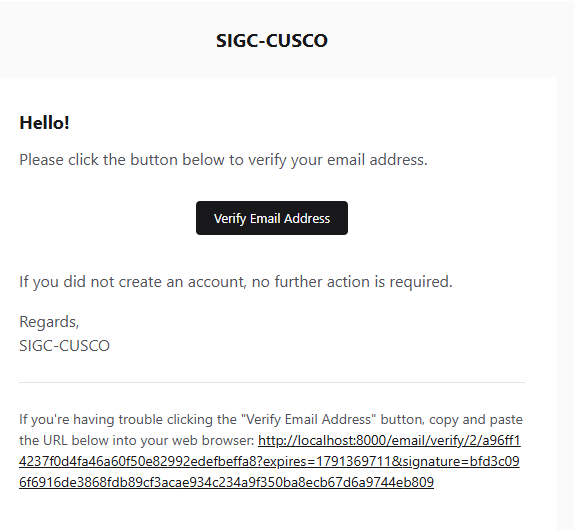
\includegraphics[width=0.9\textwidth]{captura-verificacion-correo.png}
    \caption{Correo de verificación enviado por SIGC-CUSCO.}
    \label{fig:correo-verificacion}
\end{figure}

En la \cref{fig:correo-verificacion} se observa el botón \enquote{Verify Email
Address} y el enlace alternativo que puede copiarse en el navegador. El enlace
se genera de forma temporal para evitar que la confirmación permanezca válida
indefinidamente.

\begin{cajaevidencia}{Capturas de pantalla del sistema}
    \textbf{¿Qué debe ingresar aquí?:}
    Capturas de pantalla de la aplicación web: formulario de login, formulario para crear una capacitación y tabla de cursos guardados en la base de datos.
    \vspace{0.15cm}
    \textbf{Ejemplo sugerido:}
    Pegar una o dos imágenes mostrando la pantalla de login y el listado de capacitaciones activas en \texttt{http://localhost:8000/cursos}.
\end{cajaevidencia}

\subsubsection{Pruebas o validaciones realizadas}
Se implementó una suite integral de pruebas automáticas con Pest PHP y PHPUnit sobre una base de datos MySQL dedicada (\texttt{SIGC\_testing}), garantizando el aislamiento del entorno de producción y desarrollo:

\begin{table}[H]
\centering
\small
\begin{tabularx}{\textwidth}{P{1.8cm} P{4.8cm} P{4.5cm} Y}
\toprule
\textbf{Código} & \textbf{Prueba realizada} & \textbf{Resultado esperado} & \textbf{Estado} \\
\midrule
\textbf{CP-01} & Alumno intenta entrar a la pantalla de crear cursos. & Acceso denegado (Error HTTP 403 vía \texttt{CoursePolicy}). & \textbf{Aprobado} \\
\addlinespace
\textbf{CP-02} & Se intenta guardar un curso con vacantes en 0 o negativo. & Formulario bloquea y muestra mensaje de alerta en español. & \textbf{Aprobado} \\
\addlinespace
\textbf{CP-03} & Se ingresa una fecha de fin menor a la fecha de inicio. & Error de validación por fechas incoherentes (\texttt{after\_or\_equal}). & \textbf{Aprobado} \\
\addlinespace
\textbf{CP-04} & Se completa el formulario con datos válidos y docente. & Curso persistido en base de datos MySQL y visible en catálogo. & \textbf{Aprobado} \\
\addlinespace
\textbf{CP-05} & Consulta de DNI mediante servicio externo PeruDevs. & Retorna objeto estructurado \texttt{DniPerson} y almacena en caché 30 días. & \textbf{Aprobado} \\
\bottomrule
\end{tabularx}
\caption{Pruebas automáticas ejecutadas en el Incremento 1.}
\label{tab:pruebas_inc1}
\end{table}

\paragraph{Resultado de ejecución de la suite de pruebas.}
A continuación se reporta la ejecución de la batería completa de pruebas automatizadas:

\begin{quote}
    \texttt{\$ php artisan test} \\
    \texttt{Tests\textbackslash Feature\textbackslash Auth\textbackslash RegistrationTest ................. PASS} \\
    \texttt{Tests\textbackslash Feature\textbackslash CourseTest ................................... PASS} \\
    \texttt{  [OK] no autenticado o no admin no puede acceder a crear cursos} \\
    \texttt{  [OK] capacidad debe ser un entero positivo} \\
    \texttt{  [OK] fecha de fin debe ser posterior o igual a fecha de inicio} \\
    \texttt{  [OK] admin puede registrar curso valido en mysql} \\
    \texttt{  [OK] endpoint dni retorna 422 para dni invalido} \\
    \texttt{Tests\textbackslash Feature\textbackslash Services\textbackslash DniLookupServiceTest ............ PASS} \\
    \texttt{  [OK] consulta exitosa retorna DniPerson estructurado} \\
    \texttt{  [OK] respuesta exitosa se almacena en cache 30 dias} \\
    \texttt{\textbf{Tests: 50 passed (166 assertions)}} \\
    \texttt{Duration: 2.50s}
\end{quote}

\subsubsection{Cambios realizados respecto al avance anterior}
\begin{itemize}[nosep]
    \item \textbf{Uso formal de Jira:} Se abandonaron notas externas para controlar cada tarea con tickets de Jira (\texttt{SIGC-XX}).
    \item \textbf{Tablas ordenadas en MySQL:} Se separaron las tablas de usuarios, roles y cursos para no duplicar datos y asegurar relaciones limpias.
    \item \textbf{Validación estricta en Laravel:} Se configuraron reglas automáticas para impedir que se ingresen cupos negativos o fechas erróneas.
\end{itemize}

\subsubsection{Métricas y seguimiento del proceso}
\begin{itemize}[nosep]
    \item \textbf{Tiempo por tarea (\textit{Cycle Time}):} En promedio, cada historia tomó 2 días desde que se empezó a programar hasta que se aprobó.
    \item \textbf{Control de tareas en curso:} Se respetó el tope de 2 tareas simultáneas, evitando amontonar trabajo sin terminar.
    \item \textbf{Cumplimiento:} Se terminaron al 100\% las dos historias comprometidas (\texttt{SIGC-1} y \texttt{SIGC-2}).
\end{itemize}

\begin{cajaevidencia}{Captura del tablero Jira}
    \textbf{¿Qué debe ingresar aquí?:}
    Captura de pantalla de Jira mostrando las tarjetas en la columna \textbf{Done} (Hecho).
    \vspace{0.15cm}
    \textbf{Ejemplo sugerido:}
    Pegar imagen del tablero mostrando los tickets \texttt{SIGC-1} (Roles) y \texttt{SIGC-2} (Cursos) en la columna \textbf{Done}.
\end{cajaevidencia}

\subsubsection{Acuerdos de mejora para el siguiente incremento}
\begin{enumerate}[nosep]
    \item \textbf{Revisión rápida de código:} Atender los Pull Requests en menos de 24 horas para no frenar a los compañeros.
    \item \textbf{Escribir pruebas antes del código:} Aplicar TDD para la matrícula de alumnos y control de aforo antes de diseñar la pantalla.
    \item \textbf{Alistar la lectura de QR:} Probar la librería de escaneo con cámara antes de empezar el segundo incremento.
\end{enumerate}

\vspace{0.3cm}

% 7. Política de uso de IA y registro de uso
\section{Política de uso de IA y registro de uso}

En SIGC-CUSCO la Inteligencia Artificial se utiliza como una herramienta de apoyo para consultas técnicas. La autoría y responsabilidad del software es 100\% del equipo de estudiantes.

\subsection{Política de uso de IA}

\begin{itemize}[nosep]
    \item \textbf{Uso permitido:} Ayuda para ordenar historias de usuario, consultas puntuales de sintaxis en Laravel 13 y sugerencias de casos de prueba para PHPUnit.
    \item \textbf{Uso prohibido:} Copiar y pegar código sin revisarlo; dejar que la IA decida la estructura del sistema o la base de datos; y subir datos privados o contraseñas a herramientas públicas.
    \item \textbf{Regla obligatoria:} Toda ayuda de la IA debe probarse con PHPUnit y revisarse en equipo antes de integrarla al proyecto.
\end{itemize}

\subsection{Registro de uso de IA (Bitácora)}

\begin{table}[H]
\centering
\small
\begin{tabularx}{\textwidth}{P{2.2cm} P{2.6cm} P{4.2cm} Y}
\toprule
\textbf{Fecha / Ticket} & \textbf{Herramienta} & \textbf{¿Qué se consultó?} & \textbf{¿Cómo se revisó y aprobó?} \\
\midrule
\textbf{28/09/2026} \newline \texttt{SIGC-1} & Claude 3.5 Sonnet & Mejorar redacción de historias de usuario para roles en formato Gherkin. & Se quitaron supuestos que no pedía el docente y se subieron a Jira. \textit{Revisó: N. Choquenaira.} \\
\addlinespace
\textbf{02/10/2026} \newline \texttt{SIGC-2} & ChatGPT (GPT-4o) & Sintaxis de validación en Laravel para que la fecha final no sea antes del inicio. & Se usó la regla nativa de Laravel y se probó con el caso CP-03. \textit{Revisó: C. Ccama.} \\
\addlinespace
\textbf{07/10/2026} \newline \texttt{SIGC-3} & Google Antigravity & Diseño de servicio desacoplado y caché para la API REST de DNI PeruDevs. & Se implementó el contrato \texttt{DniLookupService}, DTO inmutable y se validó con suite de pruebas Pest. \textit{Revisó: F. Choquenaira.} \\
\bottomrule
\end{tabularx}
\caption{Bitácora de consultas técnicas a Inteligencia Artificial.}
\label{tab:registro_ia}
\end{table}

\vspace{0.15cm}

% 8. Conclusiones
\section{Conclusiones}

\begin{enumerate}
    \item \textbf{Organización ágil efectiva:} La combinación de ciclos cortos de Scrum, el tablero con límites de Kanban y las pruebas de XP permitieron al equipo de tres estudiantes coordinarse bien y entregar el primer incremento en el plazo de dos semanas.

    \item \textbf{Base técnica sólida:} El uso de Laravel 13 junto con MySQL 8.0 aseguró que los datos de usuarios, roles y cursos se guarden de manera ordenada, evitando inconsistencias en los cupos y facilitando la seguridad del sistema.

    \item \textbf{Disciplina de trabajo en Jira:} Poner un límite de máximo dos tareas a la vez ayudó a que el equipo no se disperse y obligó a revisar y cerrar el código antes de comenzar cosas nuevas.

    \item \textbf{Uso responsable de la IA:} Utilizar la Inteligencia Artificial solo como apoyo para consultas rápidas ahorró tiempo, manteniendo siempre el control del código mediante pruebas automáticas y revisión manual entre compañeros.
\end{enumerate}


\end{document}
